
\chapter{Τεχνικές μείωσης της πολυπλοκότητας του αλγορίθμου \textlatin{LLE}}
\par
Το σημαντικότερο αποτέλεσμα της εργασίας αυτής είναι οι δύο συνδυαστικές μέθοδοι που προτείνονται με τις οποίες μπορεί κάποιος να αποφύγει το τεράστιο υπολογιστικό κόστος που απαιτείται για την εκτέλεση του αλγορίθμου. Συγκεκριμένα το τελευταίο βήμα του αλγορίθμου το οποίο είναι και το πιο απαιτητικό έχει πολυπλοκότητα $\mathcal{O}(N^{3})$ στην γενική περίπτωση ενώ στην συγκεκριμένη περίπτωση λόγω του αραιού μητρώου $M$ είναι της τάξης $\mathcal{O}(N^{2})$. Αντιλαμβανόμαστε λοιπόν ότι ακόμα και για ένα σχετικά μικρό σετ δεδομένων, για τα δεδομένα του κλάδου της μηχανικής μάθησης, το πρόβλημα που έχουμε να αντιμετωπίσουμε έχει απαγορευτικές διαστάσεις. 
\par
Ένα άλλο πρόβλημα που συναντάει κανείς κατά την εφαρμογή του αλγορίθμου σε κάποιο σετ δεδομένων είναι ο εξής περιορισμός. Ας υποθέσουμε ότι έχουμε ένα σύνολο δεδομένων μεγέθους $N$, από τα οποία για κάποιον αριθμό $N1$ από αυτά γνωρίζουμε την ετικέτα τους. Με τον όρο ετικέτα εννοούμε την τελική κλάση στην οποία ανήκει το κάθε δείγμα. Για τα υπόλοιπα δείγματα, έστω μεγέθους $N2$ δεν γνωρίζουμε την ετικέτα τους και είναι αυτά τα δείγματα για τα οποία θέλουμε να εξάγουμε το συμπέρασμα. Το συμπέρασμα αυτό είναι φυσικά η τελική απόφαση ως προς σε ποια κλάση θα πρέπει να ταξινομηθεί το καθένα από αυτά. Προφανώς η παραπάνω απόφαση προκύπτει λαμβάνοντας υπόψιν την πληροφορία την οποία μας δίνει το σύνολο των δεδομένων $N1$ τα οποία στον χώρο της μηχανικής μάθησης αναφέρονται ως το σύνολο των δεδομένων εκπαίδευσης \textlatin{(train data)}. Τα υπόλοιπα δείγματα $N2$ αναφέρονται ως το σύνολο των δεδομένων αξιολόγησης \textlatin{(test data)}.
\par
Στο συγκεκριμένο λοιπόν έστω ότι τα δείγματα του αρχικού χώρου έχουν αρχική διάσταση μεγέθους $D$ και μέσω του αλγόριθμου μείωσης των διαστάσεων θέλουμε να βρεθούμε σε έναν νέο χώρο διάστασης $d$, προφανώς με $d < D$. Στην περίπτωση αυτή λοιπόν ο πιο απλός συλλογισμός που θα μπορούσε να κάνει κάποιος είναι να εφαρμόσει τον αλγόριθμο \textlatin{LLE} πάνω στο σετ δεδομένων εκπαίδευσης ώστε να έχει ένα σύνολο δεδομένων μεγέθους $Ν1$, διάστασης $d$. Με τον ίδιο ακριβώς τρόπο θα μπορούσε να έχει και το δεύτερο σετ δεδομένων, τα δεδομένα αξιολόγησης, μεγέθους $N2$ και αυτά διάστασης $d$. Έπειτα για την ταξινόμηση των αποτελεσμάτων θα μπορούσε να εφαρμοστεί ο αλγόριθμος ταξινόμησης κοντινότερων γειτόνων ανάμεσα στο σετ αξιολόγησης με το σετ εκπαίδευσης. Στη συνέχεια ανάλογα με την κλάση στην οποία ανήκει ο κοντινότερος γείτονας από το σετ εκπαίδευσης για κάθε ένα στοιχείο των δεδομένων αξιολόγησης, θα καταλήγαμε στην τελική απόφαση για την κλάση στην οποία ανήκει κάθε ένα από τα δεδομένα του σετ $N2$. Προφανώς ο αλγόριθμος κοντινότερων γειτόνων θα εφαρμοσθεί στον χώρο μειωμένης διάστασης μεγέθους $d$ χρησιμοποιώντας για παράδειγμα την μετρική της Ευκλείδειας απόστασης μεταξύ των σημείων.
\par
Αν λοιπόν εφαρμόσουμε την παραπάνω διαδικασία για κάποιο σετ δεδομένων, θα παρατηρήσουμε ότι το τελικό αποτέλεσμα της ταξινόμησής μας έχει πολύ μικρή επιτυχία. Αυτό συμβαίνει διότι, οι δύο υποχώροι οι οποίοι προέκυψαν από το τελικό βήμα του αλγορίθμου \textlatin{LLE}, κατά το οποίο υπολογίστηκε ο νέος χώρος μειωμένης διάστασης για κάθε ένα από τα δύο σύνολα δεδομένων, έχουν διαφορετική διανυσματική βάση και δεν μπορούν σε καμιά περίπτωση να συσχετιστούν μεταξύ τους ώστε να μπορέσουμε από τα δεδομένα του ενός να καταλήξουμε σε κάποιο ορθό συμπέρασμα για τα δεδομένα του άλλου. Ο παραπάνω λοιπόν περιορισμός μας αναγκάζει να εφαρμόσουμε τον αλγόριθμο μείωσης των διαστάσεων στο σύνολο των δεδομένων, δηλαδή δίνοντας σαν είσοδο στον αλγόριθμο το σύνολο των δεδομένων μεγέθους $N = N1+N2$. Με τον τρόπο αυτό θα καταλήγαμε σε ένα νέο σετ δεδομένων μεγέθους $N$ αλλά διάστασης $d < D$. Τέλος σε αυτό το σετ δεδομένων μπορούμε τώρα να εφαρμόσουμε τον αλγόριθμο εύρεσης κοντινότερων γειτόνων για κάθε ένα απο τα δεδομένα αξιολόγησης ως προς τα δεδομένα εκπαίδευσης, φυσικά στον χώρο $d$ διαστάσεων, και έτσι να καταλήξουμε στην ορθή ταξινόμηση των δειγμάτων $N2$ ως προς την κλάση στην οποία ανήκουν. 

\section{Μέθοδοι αντιμετώπισης της πολυπλοκότητας του προβλήματος}
\par
Όπως αντιλαμβανόμαστε από την παραπάνω ανάλυση, η διαδικασία αυτή δεν είναι καθόλου πρακτική και μάλιστα δεν δίνει την δυνατότητα για λήψη αποφάσεων και ταξινόμησης δειγμάτων σε πραγματικό χρόνο. Αυτό διότι, για κάθε δείγμα αξιολόγησης που μας έρχεται ως είσοδος κάποια συγκεκριμένη χρονική στιγμή, και για το οποίο θέλουμε να το ταξινομήσουμε σε κάποια κλάση, θα πρέπει να το ενσωματώνουμε στο σετ των δεδομένων εκπαίδευσης και στην συνέχεια να εκτελούμε τον αλγόριθμο \textlatin{LLE}. Η συγκεκριμένη διαδικασία δεν προσφέρεται σε καμιά περίπτωση για πρακτικές εφαρμογές κατά τις οποίες μάλιστα ο στόχος μας είναι να γίνει μείωση των διαστάσεων ώστε να μπορούμε να λαμβάνουμε ταχύτερα και ακριβέστερα αποτελέσματα. Το γεγονός αυτό μάλιστα αντιτίθεται στην συνολική φιλοσοφία της μείωσης των διαστάσεων κατά την οποία μέσω της εφαρμογής της μπορεί να επιταχυνθεί σε πολύ μεγάλο βαθμό η διαδικασία της ταξινόμησης.

\subsection{Μέθοδος-1: Προβολή στον χώρο των δεδομένων εκπαίδευσης}
\par
Για τους λόγους λοιπόν οι οποίοι αναλύθηκαν παραπάνω, προκύπτει η ανάγκη να βρεθεί κάποιος τρόπος με τον οποίο να μπορούμε οποιαδήποτε στιγμή να ταξινομήσουμε κάποιο δεδομένο, χρησιμοποιώντας βέβαια την πληροφορία που μπορούν να μας δώσουν τα δεδομένα του σετ εκπαίδευσης. Την λύση στο πρόβλημα αυτό λοιπόν έρχεται να δώσει η λογική με την οποία λειτουργεί ο αλγόριθμος \textlatin{LLE}. Πιο συγκεκριμένα όπως αναφέραμε παραπάνω, η μέθοδος αυτή έχει ως στόχο να διατηρήσει τα γεωμετρικά τοπικά χαρακτηριστικά για κάθε ένα από τα δείγματα του συνόλου εκπαίδευσης τόσο στον χώρο των αρχικών διαστάσεων όσο και στον τελικό χώρο μειωμένης διάστασης. Επίσης, λόγω του ότι η ενσωμάτωση των δεδομένων στον χώρο μειωμένης διάστασης γίνεται με τη χρήση του πίνακα βαρών $W$, ο οποίος προσδιορίζει για κάθε δείγμα του αρχικού χώρου την ανακατασκευή του μέσω των κοντινών του γειτόνων προκύπτει και η ιδέα της μεθόδου αυτής. Ο αντίστοιχος ψευδοκώδικας είναι ο παρακάτω
\selectlanguage{english}
\begin{algorithm}
   \caption{Projection Method}
    \begin{algorithmic}[1]   	
    	\State Let $Xtrain$ be $[D \times N1]$ Train\textunderscore dataset matrix and $Xtest$ be $[D \times N2]$ Test\textunderscore dataset matrix \Comment{N1,N2 declare the number of data and D the number of dimensions}
		\State 
    	
    	\State Let matrix $Y$ be $[d \times N1]$ Train data, after dimensionality reduction \Comment{ d < D}
    	\State
    	
    	\State Let matrix nn\textunderscore graph with size $[N1 \times N2]$ and all elements equal to zero
    	\State 
        
        \For{$i = 1$ to ${N_2}$}
            \State Find K-Nearest Neighbors from $Xtrain$
        \EndFor
        \State
		
		\State Keep the results to matrix IDX with size $[N2 \times K]$ \Comment{ K is the number of nearest neighbors}
		\For{$i = 1$ to ${N_2}$}
            \State Set IDX(i,1:K) cells of nn\textunderscore graph matrix equal to ones
            \State Make the matrix multiplication $Y \times$ nn\textunderscore graph$(1:N1,i)$ and store the result to \\ $testY(1:d,i)$ \Comment{testY(:,i) is the result of dimensionality reduced $Xtest_i$}
        \EndFor
        \State 
        
        \State Final matrix testY has size $[d \times N2]$ and represents the projection of Xtest D-dimensional data into the d-dimensional emndedding subspace.  
        \State
        \State Now execute K-NN Classification between testY and Y datasets, to the d-dimensional space
	\end{algorithmic}
\end{algorithm}
\selectlanguage{greek}
\par
Από την παραπάνω ανάλυση της μεθόδου γίνεται φανερό ότι μπορούμε να χρησιμοποιήσουμε την πληροφορία των δεδομένων \textlatin{Y}, τα οποία είναι τα δεδομένα εκπαίδευσης \textlatin{Xtrain} στον χώρο μειωμένης διάστασης, ώστε να ταξινομήσουμε οποιοδήποτε δείγμα από το σετ δεδομένων αξιολόγησης. Το γεγονός αυτό, σε συνδυασμό με την ελάχιστη αύξηση του σφάλματος ταξινόμησης όπως θα γίνει φανερό στα αποτελέσματα των πειραμάτων κάνει την μέθοδο αυτή πολύ ελκυστική για πρακτικές εφαρμογές. Τέτοιες εφαρμογές απαιτούν αποτελέσματα σε πραγματικό χρόνο και μάλιστα σε πολύ μεγάλες ταχύτητες γεγονός το οποίο εξασφαλίζεται από τους υπολογισμούς στον χώρο των μειωμένων διαστάσεων $d$. Όπως μπορούμε να παρατηρήσουμε στο πρώτο βήμα της μεθόδου εφαρμόζουμε τον αλγόριθμο κοντινότερων γειτόνων στον χώρο των αρχικών διαστάσεων μεγέθους $D$, για το σετ δεδομένων αξιολόγησης ως προς το σετ δεδομένων εκπαίδευσης. Επομένως θα μπορούσαμε να ισχυριστούμε ότι το υπόλοιπο της διαδικασίας είναι περιττό εκτός και αν το τελικό αποτέλεσμα ταξινόμησης είναι καλύτερο από αυτό στον αρχικό χώρο. Παρόλα αυτά αν αναλογιστούμε ένα πολύ μεγάλο σετ δεδομένων με έναν αρκετά μεγάλο αριθμό διαστάσεων, όπως πρόκειται άλλωστε για τα περισσότερα πραγματικά σετ στον χώρο της αναγνώρισης προτύπων, τότε το γεγονός ότι από το σημείο αυτό και μετά μπορούμε την πληροφορία των $D$ διαστάσεων να την πάρουμε από τις πολύ λιγότερες όπως θα δούμε $d$ τελικές διαστάσεις αποτελεί τεράστιο κέρδος. Το κέρδος είναι τόσο σε κόστος υπολογισμού πχ σε κάποιον υπολογιστικά ακριβό αλγόριθμο στην συνέχεια της ροής του προγράμματος μας όσο και στους απαραίτητους πόρους μνήμης που απαιτούνται για την διαχείριση των δεδομένων.  
\par
Στην παραπάνω διαδικασία θεωρήσαμε ότι έχουμε ήδη εφαρμόσει τον αλγόριθμο \textlatin{LLE} στο σετ δεδομένων εκπαίδευσης και έτσι έχουμε το αποτέλεσμα, δηλαδή τα δεδομένα στον χώρο μειωμένης διάστασης στον πίνακα \textlatin{Y}. Το βήμα αυτό, παρότι είναι σαφώς οικονομικότερο από την περίπτωση στην οποία θα εφαρμόζαμε στον αλγόριθμο στο σύνολο των δεδομένων εκπαίδευσης αλλά και των δεδομένων αξιολόγησης, στις περισσότερες εφαρμογές απαιτεί πολύ μεγάλο μέγεθος μνήμης γεγονός που καθιστά τις περισσότερες φορές αδύνατη την εκτέλεση του αλγορίθμου. Για να διευκρινιστεί η διαδικασία εφαρμογής της μεθόδου αλλά και οι διαστάσεις των πινάκων κάθε βήματος δίνεται το παρακάτω διάγραμμα  
\newpage
\begin{figure}[H]
\centering
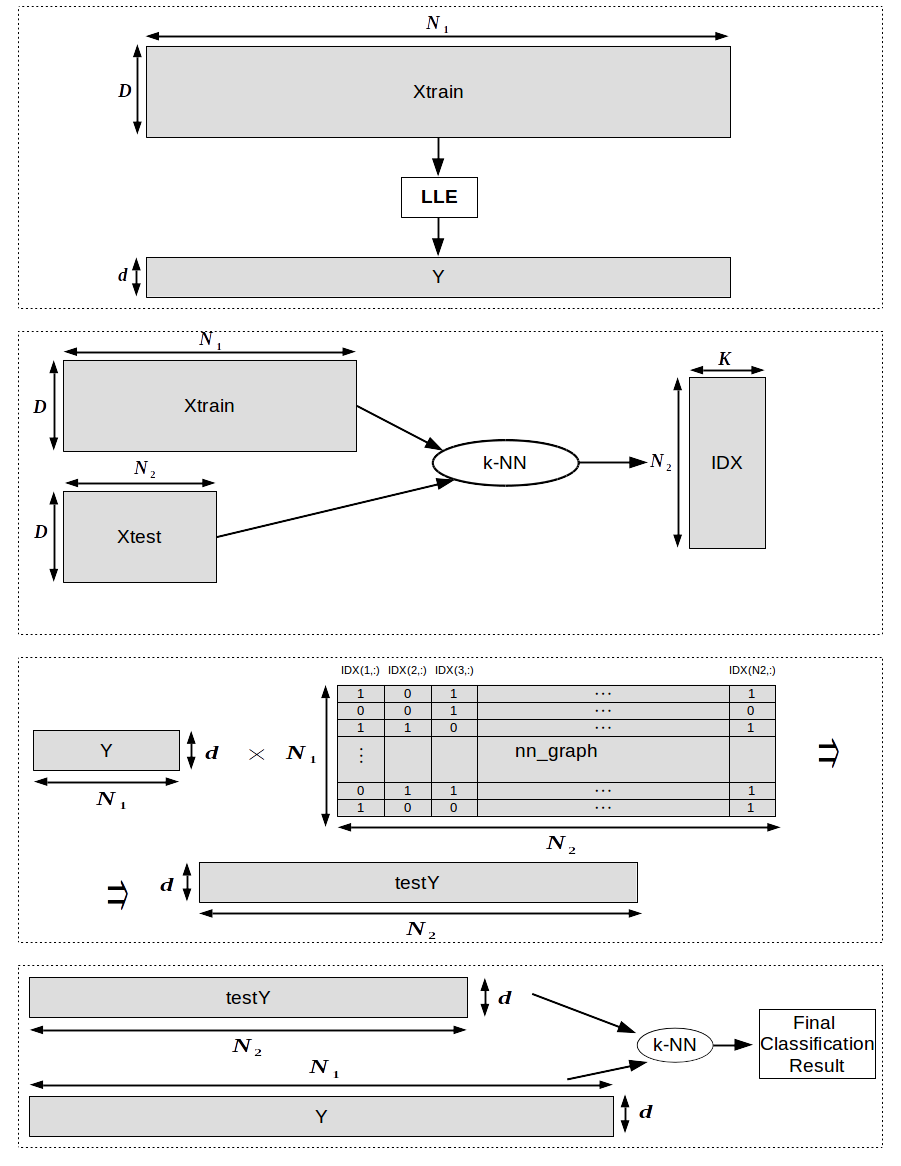
\includegraphics[scale=0.8]{figs/5.png}
\newline
\caption{ Μέθοδος-1: Προβολή των δεδομένων αξιολόγησης στον χώρο των δεδομένων εκπαίδευσης. } 
\end{figure}
\newpage

\subsection{Μέθοδος-2: Δημιουργία υποσυνόλων και πλειοψηφική απόφαση ταξινόμησης }
\par
Για την αντιμετώπιση λοιπόν του παραπάνω προβλήματος μπορούμε να εφαρμόσουμε την Μέθοδο-2. Η βασική ιδέα της μεθόδου αυτής, όπως θα δούμε αναλυτικά και στον ψευδοκώδικα παρακάτω, είναι να διασπάσει το αρχικό σετ δεδομένων σε υποσύνολα από τα οποία στην συνέχεια συνδυάζει την πληροφορία που δίνει το καθένα και εξάγει το τελικό αποτέλεσμα ταξινόμησης. Σημαντικό σημείο στην διαδικασία αυτή είναι η κατασκευή των υποσυνόλων να γίνει με τρόπο τέτοιο ώστε το καθένα από αυτά να περιέχει την ίδια ποσότητα πληροφορίας, με την έννοια ότι θα πρέπει ο διαμοιρασμός των δειγμάτων κάθε κλάσης να γίνει ομοιόμορφα σε όλα τα υποσύνολα. Με τον τρόπο αυτό στην πραγματικότητα επιλύονται πολλά μικρά υποπροβλήματα όμοια με το αρχικό. Υποπροβλήματα δηλαδή τα οποία περιέχουν την ίδια πληροφορία με το αρχικό σετ δεδομένων εκπαίδευσης αλλά σε μικρότερη ποσότητα. Αν προσέξουμε ώστε το κάθε υποσύνολο να περιέχει αρκετά δείγματα ώστε να μπορέσει να διατηρηθεί το λείο της πολλαπλότητας το οποίο είναι απαίτηση του αλγορίθμου \textlatin{LLE} τότε το αποτέλεσμα της λύσης κάποιου υποχώρου θα είναι πολύ κοντά σε αυτό του αρχικού προβλήματος. Συνδυάζοντας την πληροφορία των υποχώρων στη συνέχεια, και καταλήγοντας στο αποτέλεσμα της ταξινόμησης ανάλογα με την πλειοψηφία των αποτελεσμάτων όλων των υποχώρων το κέρδος είναι διπλό. Μειώνεται καταρχήν δραματικά το κόστος υπολογισμού του αλγορίθμου \textlatin{LLE} λόγω της μείωσης κατά μεγάλο βαθμό των δειγμάτων στα οποία εφαρμόζεται. Επίσης με την διαδικασία του ψηφίσματος και της πλειοψηφικής τελικής επιλογής βελτιώνεται κατά πολύ το αποτέλεσμα της ταξινόμησης σε σχέση με αυτό του κάθε υποχώρου ξεχωριστά. 
\par
Για να γίνει κατανοητός ο τρόπος κατασκευής των υποσυνόλων αλλά και της συνολικής διαδικασίας της μεθόδου δίνεται ένα γράφημα το οποίο αναπαριστά τον διαμοιρασμό των δειγμάτων και έπειτα ο συνολικός ψευδοκώδικας της μεθόδου. Στο παρακάτω γράφημα έστω ότι το αρχικό μου σύνολο δεδομένων είναι το γνωστό σύνολο δεδομένων \textlatin{MNIST}\textlatin{\cite{mnist}} με μέγεθος \textlatin{N} και το οποίο περιέχει δεδομένα τα οποία ανήκουν σε δέκα κλάσεις (ψηφία από το 0 έως το 9). Επίσης κάθε εικόνα έχει γίνει μετατροπή σε ένα διάνυσμα-στήλη μεγέθους $[Width \times Height]$, έστω $D$. Τέλος το συγκεκριμένο παράδειγμα επιλέγουμε να το χωρίσουμε σε 3 υποσύνολα. Η διαδικασία διαμοιρασμού των δειγμάτων φαίνεται γραφικά παρακάτω
\newpage
\clearpage
\begin{figure}[t!]
\centering
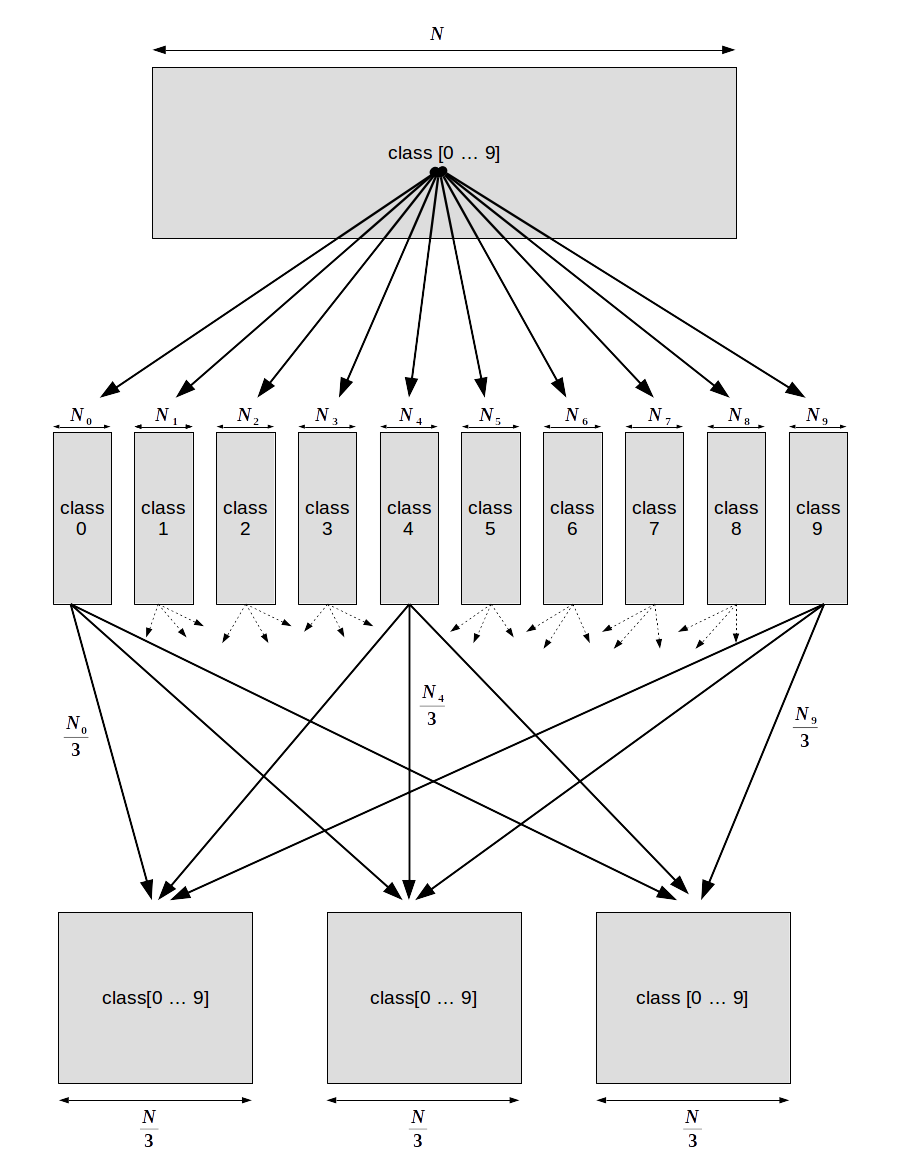
\includegraphics[scale=0.8]{figs/6.png}
\newline
\caption{ Μέθοδος-2.1: Δημιουργία των υποσυνόλων.} 
\end{figure}
\newpage
\par
Όπως φαίνεται αναλυτικά στο παραπάνω σχήμα το σύνολο των αρχικών κλάσεων ομαδοποιείται και στην συνέχεια μοιράζονται ανάλογα τα δείγματα κάθε κλάσης, ομοιόμορφα, σε όσα υποσύνολα έχουμε επιλέξει. Από το σημείο αυτό λοιπόν μπορούμε πλέον να εφαρμόσουμε τον αλγόριθμο μείωσης διστάσεων, \textlatin{LLE}, σε κάθε ένα από τα τελικά υποσύνολα δεδομένων καταλήγοντας σε τρεις νέους χώρους μειωμένης διάστασης \textlatin{d}. Να διευκρινιστεί στο σημείο αυτό ότι η διαδικασία προβολής των δεδομένων αξιολόγησης μπορεί να γίνει είτε ενσωματώνοντάς τα σε κάθε ένα από τα τρία τελικά σετ δεδομένων πριν την εφαρμογή του αλγορίθμου ή να εφαρμοστεί η Μέθοδος-1. Σύμφωνα με την Μέθοδο-1, όπως εξηγήσαμε και παραπάνω, θα γίνει μείωση των διαστάσεων για κάθε υποσύνολο και στην συνέχεια για κάθε ένα χωριστά θα γίνει η προβολή των δεδομένων αξιολόγησης στον χώρο μειωμένης διάστασης του καθενός. 
\par
Αφού εφαρμοστεί μια από τις παραπάνω μεθόδους, ανεξαρτήτως ποια, μπορούμε πλέον για κάθε ένα σύνολο δεδομένων (τελικά σετ εκπαίδευσης ένα εως τρία και σετ αξιολόγησης στον χώρο μειωμένης διάστασης $d$) να εφαρμόσουμε τον αλγόριθμο κοντινότερων γειτόνων \textlatin{(k-NN)} και να κάνουμε την ταξινόμηση κάθε δείγματος του σετ αξιολόγησης, στην κλάση εκτίμησης για κάθε έναν από τους τελικούς υποχώρους. Τέλος, πλειοψηφικά αποφασίζουμε σε ποια κατηγορία ανήκει το κάθε δείγμα, λαμβάνοντας υπόψιν την ψήφο ως προς την κλάση ταξινόμησης του δείγματος από τους τρεις υποχώρους. Με τον τρόπο αυτό, όπως θα φανεί και στα πειράματα παρακάτω, βελτιώνεται σε πολύ μεγάλο βαθμό το τελικό αποτέλεσμα της ταξινόμησης σε σχέση με αυτό των τριών υποχώρων. Η διαδικασία αυτή, παρουσιάζεται και γραφικά στο παρακάτω σχήμα
\newpage
\begin{figure}[t!]
\centering
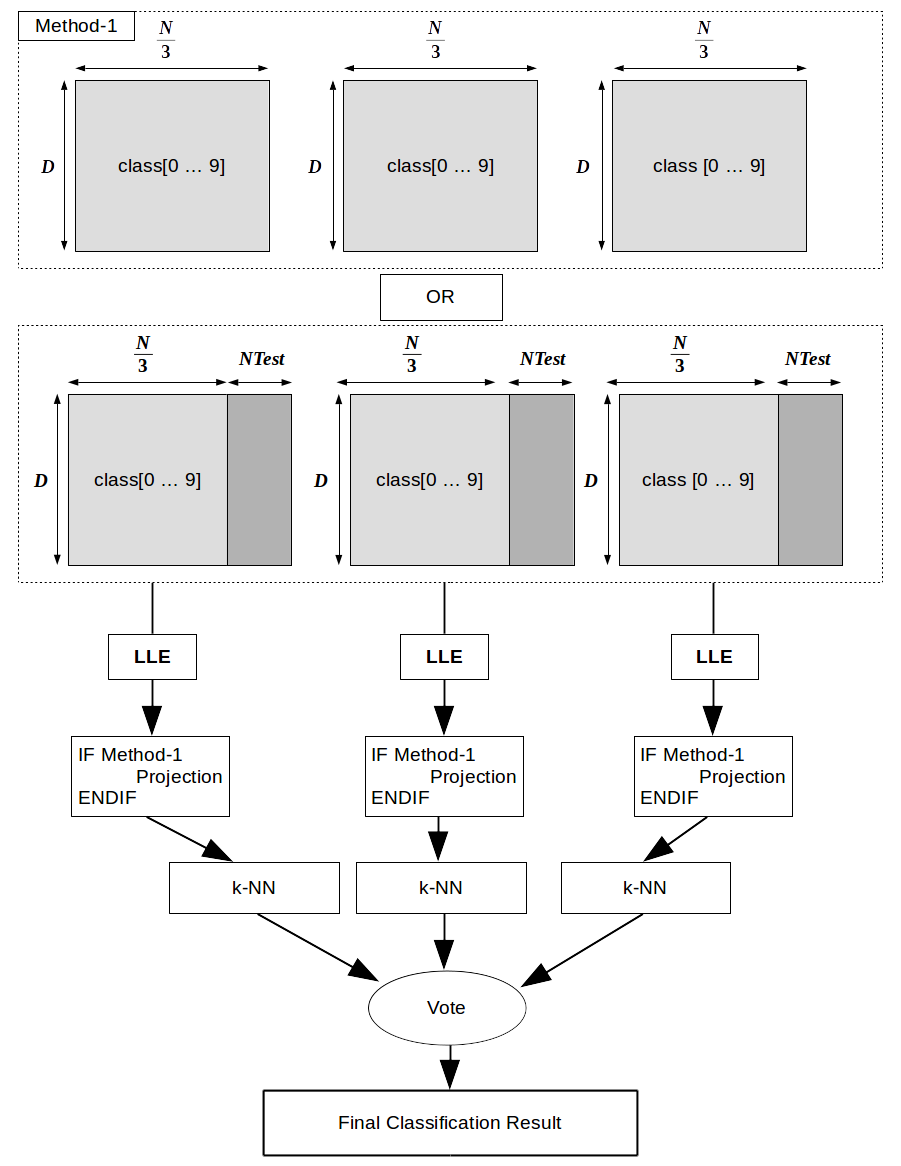
\includegraphics[scale=0.8]{figs/7.png}
\newline
\caption{ Μέθοδος-2.2: Μείωση των διαστάσεων στα υποσύνολα και πλειοψηφική απόφαση της τελικής ταξινόμησης. } 
\end{figure}
\newpage
